\documentclass{beamer}

\usepackage{amsmath,amsfonts,amssymb} %math stuff
\usepackage{graphicx}
\usepackage{comment}
\usepackage{linegoal}
\usepackage{tikz}
\usepackage{ifthen}
\usepackage{progressbar}
\usepackage{natbib}
\usetikzlibrary{calc}
\usepackage{algorithm}
\usepackage{algorithmic}
\usepackage{soul}
\usepackage{xspace}

%\usepackage{animate}


\newcommand{\ZZ}{{\mathbb{Z}}} \newcommand{\QQ}{{\mathbb{Q}}}
\newcommand{\RR}{{\mathbb{R}}} \newcommand{\CC}{{\mathbb{C}}}
\newcommand{\NN}{{\mathbb{N}}} \newcommand{\KK}{{\mathbb{K}}}
\newcommand{\FF}{{\mathbb{F}}}
\newcommand{\GG}{\ensuremath{\mathcal{G}}}

%Specially for this paper:
\newcommand{\uX}{{\underline{X}}}
\newcommand{\uD}{{\underline{D}}}
\newcommand{\undlnn}{{\underline{n}}}
\newcommand{\uTheta}{{\underline{\theta}}}
\newcommand{\uZero}{{\underline{0}}}
\newcommand{\lm}{{\mathrm{lm}}}
\newcommand{\lc}{{\mathrm{lc}}}
\newcommand{\lexp}{{\mathrm{lexp}}}
\newcommand{\gcrd}{{\mathrm{GCRD}}}
\newcommand{\gcld}{{\mathrm{GCLD}}}
\newcommand{\lclm}{{\mathrm{LCLM}}}
\newcommand{\lcrm}{{\mathrm{LCRM}}}
\newcommand{\lcm}{{\mathrm{lcm}}}
\newcommand{\ncfactor}{\texttt{ncfactor.lib}\xspace}
\newcommand{\nth}{$n^{\mathrm{th}}$\xspace}

\newtheorem{remark}{Remark}

\setbeamertemplate{footline}[frame number] %For frame numbers


\title{Benchmarks and Quality Evaluation of CAS}
\subtitle{ACA 2016 -- Kassel -- Germany}

\author{Albert Heinle}
\institute{Symbolic Computation Group\\
David R. Cheriton School of Computer Science\\
University of Waterloo\\Canada}

\beamertemplatenavigationsymbolsempty %To remove the navigation bar

\date{2016--08--01}

%%%%%%%%%%%%%%%%%%%%%%%%%%%%%%
\begin{document}
\frame
{
  \titlepage
}

\frame
{
  \tableofcontents
}

\section{Correct Benchmarking of CAS -- Case Studies and Dangers}

\frame
{
    \begin{center}
      {\Huge{\insertsection}}
    \end{center}
}

\begin{frame}
  \frametitle{Find the Problem -- A Case Study I}
  You read in a paper a sentence like the following:
  \begin{quote}
    We presented a new implementation of algorithm
    X. Our timings show that we outperform the alternative programs when using examples we
    found in literature as
    input, and we observe that our program scales well by using
    randomly generated objects.
  \end{quote}
What is/are potential problem/s?
\pause
\begin{itemize}
%\item Time vs. memory
\item Are the scripts and outputs made available? Did the authors
  check if the outputs were correct for the random inputs?
\item Did the authors run the other programs on their machine, or
  did they just take the timings from the other paper?
\item Did the authors also check the scalability for the other programs?
\end{itemize}
\end{frame}

\begin{frame}[fragile]
  \frametitle{Find the Problem -- A Case Study II}
  Consider the following \textsc{Singular} code:
{\footnotesize{\begin{verbatim}
execute(read("singular_poly.txt"));
// File Content:
// ring R = 0,(x,y),dp;
// ideal I = *large polynomial system*;
timer = 1; int t = timer;
ideal g = yourCommand(I);
t = timer - t; print(g); print(t);
\end{verbatim}}}
What is/are potential problem/s?
\pause
\begin{itemize}
\item \textsc{Singular} sorts all input polynomials with respect to
  given monomial ordering. This may assist computations, but the
  sorting time is not taken into account.
\item \textsc{Singular} is open source, hence we know how the timer
  works. What happens if we would use \textsc{Maple} in a similar way?
\end{itemize}
\end{frame}

\begin{frame}[fragile]
\frametitle{Find the Problem -- A Case Study III}
{\footnotesize{\begin{verbatim}
Singular:                  | Maple:
===========================|===========================
ring R = 0,(x,y),lp;       | with(Groebner):
ideal I = x^2 + y^2, x + y;| F:=[x^2 + y^2, x + y];
print(groebner(I));        | print(Basis(F,plex(x,y)))
\end{verbatim}}}
What is/are potential problem/s?
\pause
\begin{itemize}
\item \textsc{Singular} computes by default not a \alert{reduced} Gr\"obner
  basis, while \textsc{Maple} in its current version always does.
\end{itemize}
\end{frame}

\frame
{
  \frametitle{Summarizing the Dangers of the Case Studies}
  \begin{itemize}
  \item Ad Case Study I: Loosing Transparency.
  \item Ad Case Study II: Overlooking crucial implementation details.
  \item Ad Case Study III: Different facets of certain computations
    are overlooked.
  \end{itemize}

  The threat of all the above points becomes larger with the number of
  different implementations available.
}

\section{Challenges  and Vision for Benchmarking in Computer Algebra}
\frame
{
    \begin{center}
      {\Huge{\insertsection}}
    \end{center}
}

\begin{frame}
\frametitle{What Makes Benchmarking for the Computer Algebra Community
Difficult?}
\begin{itemize}
\item Non-uniqueness of computation results. Sometimes checking
  results for ``equality'' is a difficult problem itself. This
  difficulty also transfers to checking the correctness of an output.
\item Many sub-communities with their own sets of problems.
\item Input formats for different computer algebra systems are
  differing a lot.
\end{itemize}
\end{frame}

\begin{frame}
\frametitle{What We Should Not Do...}
\begin{figure}
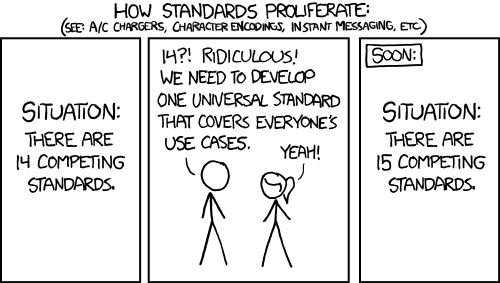
\includegraphics[width=.7\textwidth]{pics/standards.png}
\caption{Picture Taken from \url{http://xkcd.com/927/}}
\end{figure}
\end{frame}

\begin{frame}
\frametitle{\textsc{SDEval} for Benchmarking in Computer Algebra}
\begin{itemize}
\item
  \textsc{SDEval}\footnote{\url{http://wiki.symbolicdata.org/SDEval}}\footnote{\url{https://www.youtube.com/watch?v=CctmrfisZso}}
  is a benchmarking framework tailored for the computer algebra community.
\item Create Benchmarks: Using entries from the \textsc{Symbolic Data}
  database, one can create executable code for several different
  computer algebra systems.
\item Run Benchmarks: \alert<2->{Independent from the creation part}, it provides
  a feasible infrastructure to run, monitor and time computations, and
  there are interfaces for scripts to interpret the output.
\end{itemize}
\end{frame}

\begin{frame}[fragile]
  \frametitle{A Call For Transparency: The \textsc{SDEval} Solution}
  Together with papers, authors should make so-called
  \texttt{taskfolders} available. These look like the following.
\begin{figure}
{\scriptsize{
\begin{verbatim}
+ TaskFolder 
| - runTasks.py //For Running the task
| - taskInfo.xml //Saving the Task in XML Structure
| - machinesettings.xml//The Machine Settings in XML form 
| + classes //All classes of the SDEval project
| + casSources //Folder containing all executable files
| | + SomeProblemInstance1 
| | | + ComputerAlgebraSystem1
| | | | - executablefile.sdc //Executable code for CAS
| | | | - template_sol.py //Script to analyze the output of the CAS
| | | + ComputerAlgebraSystem2
| | | | - executablefile.sdc
| | | + ...
| | + SomeProblemInstance2
| | | + ...
| | + ...
\end{verbatim}}}
\caption{Folder structure of a taskfolder}
\label{fgr:TaskFolder}

\end{figure}
\end{frame}

\begin{frame}
\frametitle{What We Could be Working Towards: StarExec}
\begin{itemize}
\item StarExec\footnote{\url{https://www.starexec.org/}} is a complete
  benchmarking infrastructure for the satisfiability community
  (SAT/SMT solvers). Funded with 1.85 million USD by the NSF.
\item Different kinds of computations clearly structured and
  standardized by \textsc{SMT-LIB}.
\end{itemize}
\begin{figure}
\begin{center}
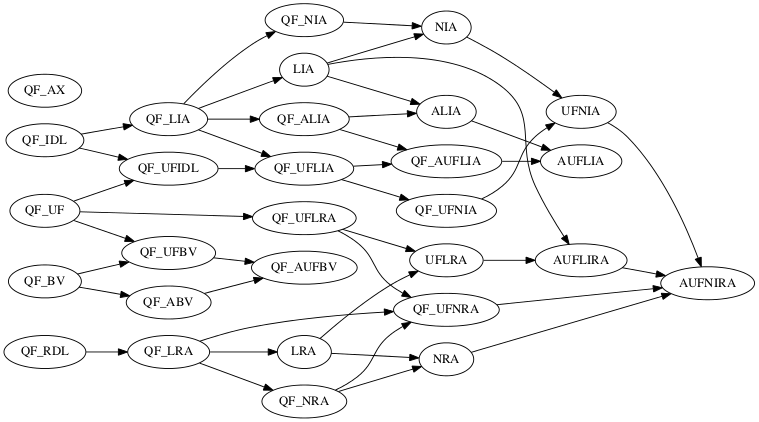
\includegraphics[width=.5\textwidth]{pics/logics.png}\\
\caption{Image taken from \url{http://smtlib.cs.uiowa.edu/logics.shtml}}
\end{center}
\end{figure}
\end{frame}

\begin{frame}
\frametitle{What We Could be Working Towards: StarExec (cntd.)}
\begin{itemize}
\item Different from \textsc{SDEval}, \textsc{StarExec} also provides
  physical computation infrastructure to perform calculations and to
  run benchmarks (Used during conferences).
\item \textsc{StarExec} does not provide the flexibility that we would
  need for computer algebra computations. However, we can learn a lot
  from their experience and maybe one day create a similar
  infrastructure for computer algebra.
\end{itemize}
\end{frame}

\section{Conclusion}
\frame
{
    \begin{center}
      {\Huge{\insertsection}}
    \end{center}
}

\begin{frame}
\frametitle{What Do We Need, What Do We Have}
\begin{itemize}
\item The computer algebra community needs to realize the need we have
  for correct, reproducible, and transparent benchmarking.
\item Several databases, like \textsc{Symbolic Data}, are available
  from different communities. We need a way to have a central overview
  of all of them.
\item With \textsc{SDEval}, we have a starting point for creating and
  running benchmarks, which can be
  refined in the future.
\item At some point, we should also introduce a computational
  infrastructure \`{a} la \textsc{StarExec}.
\end{itemize}
\end{frame}

% \bibliographystyle{apa}
% \begin{frame}[allowframebreaks]
%   \frametitle{Bibliography}
%   {\tiny{
%   \bibliography{icms2016ncfactor}}}
% \end{frame}
\end{document}
